\providecommand{\main}{../../main}
\providecommand{\figpath}[1]{\main/../lessons/#1}
\documentclass[../../main/main.tex]{subfiles}

\newdate{date}{21}{04}{2020}


\begin{document}

\chapter{Weak interactions}

\marginpar{ \textbf{Lecture 12.} \\  \displaydate{date}. \\ Compiled:  \today.}

Now we turn to the other subnuclear interaction, the weak interaction. The discussion of this topic starts from the observation of the medium lifetime of some unstable particles. QCD leads to a large spectrum of mesons and baryons, most of which are unstable with decay rates of the order of \( 100 \ \si{MeV} \), corresponding to lifetime of the order of \( 10^{-23} \ \si{s} \). However, the lightest particles of each type are more stable. Most familiarly, the neutron is unstable by \( \beta \) decay:
\begin{equation}
	n
	\longrightarrow
	pe^-\bar{\nu}_e
	\label{eq:L12_BD}
\end{equation}
though it is very long-lived:
\begin{equation}
	\tau(n)
	=
	880 \ \si{s}
	\label{eq:L12_BDL}
\end{equation}
The great difference with the typical hadronic lifetimes suggest that those particles, like neutron, decays are due to another subnuclear interaction, different from the strong one.





\section{V-A Weak Theory}
Historically, it all started with the study of \( \beta \) decay in \ref{eq:L12_BD}. Before the discovery of neutrinos, it was observed that the spectrum of \( e^- \) was continuous, but this was not possible for a two-particle product decay, i.e. \( n \longrightarrow pe^- \). Therefore, Pauli postulated the existence of a another invisible particle that enters in the products of \( \beta \) decay. Fermi called this particle \textbf{neutrino} and gave a unified description of the \( \beta \) decays of nuclei using a general 4-fermion interaction, like in Figure \ref{fig:L12_BDFD}.

\begin{figure}[!h]
	\centering
	\includegraphics[width=0.2\textwidth]{\figpath{12}/12_images/BDFD.png}
	\caption{\label{fig:L12_BDFD} Fermi description of beta decay.}
\end{figure}

Strange particles added other elements to the discussion on weak interaction. In fact, \( S \) (strangeness) is conserved in strong production of strange particles, but \( S \) must be violated in their decay. It was found:
\begin{align}
	K^0 &\xrightarrow{P=+1} \pi^+\pi^-	\\
	K^0 &\xrightarrow{P=-1} \pi^+\pi^-\pi^0
\end{align}
It seemed impossible that these decays with final state \( P=+1 \) and \( P=-1 \) could belong to the same particle, since parity was known to be an almost perfect symmetry of atomic physics and nuclear physics. In 1956, parity violation was confirmed by the experiment of Madame Wu with the study of the decay of polarized \( \text{Co}^{60} \) nuclei.

In 1958, it was proposed a model of the weak interaction based on the idea that parity is maximally violated by this type of interaction and this model was called \textbf{V-A theory}. Moreover, the V-A theory proposed that all weak interaction matrix elements could be derived from a current-current interaction of the form:
\begin{equation}
	\mathcal{M}
	=
	\left\langle
	\frac{4G_F}{\sqrt{2}} j^{\mu+}_L j_{\mu L}^{-}
	\right\rangle
	\label{eq:L12_VATME}
\end{equation}
where:
\begin{align}
	j^{\mu+}_L	&= \mu^{\dag}_L \bar{\sigma}^{\mu} e_L + u^{\dag}_L \bar{\sigma}^{\mu} d_L + \dots \label{eq:L12_JML+} \\
	j^{\mu-}_L	&= e^{\dag}_L \bar{\sigma}^{\mu} \nu_L + d^{\dag}_L \bar{\sigma}^{\mu} u_L + \dots \label{eq:L12_JML-}
\end{align}
with \( e, \mu, u, d \) representing the lepton and quark fields. What is important to observe is that only the left-handed components of the Dirac field appear in Eqs. \ref{eq:L12_JML+} and \ref{eq:L12_JML-}. The name ``V minus A'' of the theory comes from rewriting:
\begin{equation}
	u^{\dag}_L \bar{\sigma}^{\mu} D_L
	=
	\bar{u} \gamma^{\mu} \qty(\frac{1 - \gamma^5}{2}) d
	=
	\frac{1}{2} \qty[\bar{u} \gamma^{\mu} d - \bar{u} \gamma^{\mu} \gamma^5 d]
	\label{eq:}
\end{equation}
which is a difference of the \textbf{V}ector and the \textbf{A}xial vector currents. Concerning the parameter \( G_F \), it is called \textbf{Fermi constant} and it has the dimensions of \( \si{GeV^{-2}} \):
\begin{equation}
	G_F
	=
	1.166 \cdot 10^{-5} \ \si{GeV^{-2}}
	\label{eq:}
\end{equation}



\subsection{Experimental tests: muon decay}
Although V-A theory is quite simple, it makes a number of detailed and rather unexpected predictions for weak interaction processes that are confirmed by experiment.

Let's start with the muon decay. The process under study is the following:
\begin{equation}
	\mu^-
	\longrightarrow
	e^- + \bar{\nu}_e + \nu_{\mu}
	\label{eq:L12_VATMD}
\end{equation}
The Feynman diagram of the process is in Figure \ref{fig:L12_MDFD}.

\begin{figure}[!h]
	\centering
	\includegraphics[width=0.3\textwidth]{\figpath{12}/12_images/MDFD.pdf}
	\caption{\label{fig:L12_MDFD} Feynman diagram of muon decay process.}
\end{figure}

Using the various fermion fields to destroy and create initial and final particles, the matrix element is:
\begin{equation}
	\mathcal{M}
	\frac{4G_F}{\sqrt{2}}
	u^{\dag}_L(p_{\nu}) \bar{\sigma}^{\mu} u_L(p_{\mu})
	u^{\dag}_L(p_{e}) \bar{\sigma}_{\mu} v_L(p_{bar{\nu}})
	\label{eq:L12_VATMDME}
\end{equation}
From this result we can calculate the energy spectrum:
\begin{equation}
	\dv{\Gamma}{E'}
	=
	\frac{G_F^2}{12\pi^3} m^2_{\mu} E'^2 \qty(8 - \frac{4E'}{m_{\mu}})
	\label{eq:L12_VATMDES}
\end{equation}
\begin{equation}
	\Gamma
	=
	\frac{1}{\tau}
	=
	\int \d{\Gamma}
	=
	\int \d{E} \ \dv{\Gamma}{E}
	=
	\frac{G^2_F m^5_{\mu}}{192\pi^3}
	\label{eq:L12_VATMDG}
\end{equation}
where \( E' \) is the energy of \( e^- \). A plot of the results is in Figure \ref{fig:L12_MDES}.

\begin{figure}[!h]
	\centering
	\includegraphics[width=0.75\textwidth]{\figpath{12}/12_images/MDES.png}
	\caption{\label{fig:L12_MDES} Energy spectrum of positrons emitted in muon decay \( \mu^+ \longrightarrow e^+ + \bar{\nu}_{\mu} + \nu_{e} \), and comparison to the V-A prediction.}
\end{figure}

The comparison of the total rate formula with the measured value of the muon lifetime gives a very accurate value of \( G_F \):
\begin{equation}
	G_F
	=
	(1.1663787 \pm 0.0000006) \cdot 10^{-5} \ \si{GeV^{-2}}
	\label{eq:}
\end{equation}

There is one more interesting aspect of the prediction for muon decay. At the endpoint of \( e^- \) spectrum (\( x_e = 1 \)), the configuration of the electron and the neutrinos is the one in Figure \ref{fig:L12_VATMDC}.

\begin{figure}[!h]
	\centering
	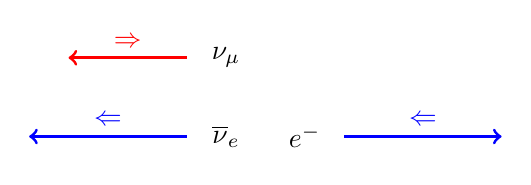
\begin{tikzpicture}[scale=1, transform shape]
		\draw [line width=.25ex,->, blue] (-1,0) -- node[above] {\( \Leftarrow \)} (-3,0);
		\draw (-0.5,0) node {\( \overline{\nu}_e \)};
		\draw [line width=.25ex,->, blue] ( 1,0) -- node[above] {\( \Leftarrow \)} ( 3,0);
		\draw ( 0.5,0) node {\( e^- \)};
		\draw [line width=.25ex,->, red] (-1,1) -- node[above] {\( \Rightarrow \)} (-2.5,1);
		\draw (-0.5,1) node {\( \nu_{\mu} \)};
	\end{tikzpicture}
	\caption{\label{fig:L12_VATMDC} Configuration of electron and neutrinos in muon decay.}
\end{figure}

The \( \nu_{\mu} \) must be left-handed, the \( \bar{\nu}_e \) must be right-handed, and the electron must be left-handed. So the angular momenta of the neutrinos cancel and the total angular momentum in the final state is carried by the electron spin. This implies that the electron must be emitted in a direction opposite to the spin of the muon. In particular, the predicted distribution for electrons at the endpoint is:
\begin{equation}
	\dv{\Gamma}{\cos \theta}
	\sim
	\qty(1 - \cos \theta)
	\label{eq:L12_VATMDED}
\end{equation}
with a maximum when the electron is moving opposite to the muon spin and a zero when the electron is parallel to the muon spin. This prediction was checked explicitly in an experiment at the TRIUMF laboratory in Vancouver, Canada, in which \( \mu^+ \)s from pion decay were stopped in an absorber and then allowed to decay. Muons from pion decay are perfectly polarized, a magnetic field was used to precess the spins of the stopped muons, and the decay electrons were counted as a function of time. The signal was seen to oscillate as the muons precess, as we can see from the data in Figure \ref{fig:L12_PDTMOS}.

\begin{figure}[!h]
	\centering
	\includegraphics[width=0.5\textwidth]{\figpath{12}/12_images/PDTMOS.png}
	\caption{\label{fig:L12_PDTMOS} Signal rates as a function of time, as the muon spin is precessed in a magnetic field, in the TRIUMF measurement of the correlation of the positron direction with the muon spin.}
\end{figure}



\subsection{Experimental tests: pion decay}
The processes we are studying now is:
\begin{align}
	\pi^- &\longrightarrow \mu^-\bar{\nu}_{\mu}	\\
	\pi^- &\longrightarrow e^-\bar{\nu}_{e}
\end{align}
According to the V-A theory, the electron and the muon have identical weak interactions. However, the ratio of branching ratios for these processes is observed to be:
\begin{equation}
	\frac{\Gamma(\pi^- \longrightarrow e^-\bar{\nu}_{e})}{\Gamma(\pi^- \longrightarrow \mu^-\bar{\nu}_{\mu})}
	=
	1.23 \cdot 10^{-4}
	\label{eq:L12_VATPDBR}
\end{equation}
%TODO ho scritto molte cazzate
Why is this happening and hiw can this be consistent with the V-A theory? The reason hides in the characteristics of the decay. The pion has spin 0, so in the decay we have in one side the electron, in the other side the antineutrino, which is right-handed. So the electron should be right-handed in order to have the momentum conserved. So the electron has the wrong helicity and the same is true also for the muon. What is making the difference? The difference comes from the mass. If we calculate the decay rate for the two cases, we find:
\begin{align}
	\Gamma(\pi^- \rightarrow \mu^-\bar{\nu}_{\mu})
	&=
	\frac{G^2_F f^2_{\pi} m^3_{\pi}}{4\pi} \frac{m^2_{\mu}}{m^2_{\pi}} \qty(1 - \frac{m^2_{\mu}}{m^2_{\pi}})^2
	\\
	\Gamma(\pi^- \rightarrow e^-\bar{\nu}_{e})
	&=
	\frac{G^2_F f^2_{\pi} m^3_{\pi}}{4\pi} \frac{m^2_{e}}{m^2_{\pi}} \qty(1 - \frac{m^2_{e}}{m^2_{\pi}})^2
\end{align}
So, the ratio of the branching ratio is equal to:
\begin{equation}
	\frac{\Gamma(\pi^- \longrightarrow e^-\bar{\nu}_{e})}{\Gamma(\pi^- \longrightarrow \mu^-\bar{\nu}_{\mu})}
	=
	\frac{m^2_e}{m^2_{\mu}} \qty(\frac{m^2_{\pi} - m^2_{e}}{m^2_{\pi} - m^2_{\mu}})^2
	=
	1.28 \cdot 10^{-4}
	\label{eq:L12_VATPDBR_2}
\end{equation}
in good agreement with the measured value quoted in \ref{eq:L12_VATPDBR}.

\end{document}
